\documentclass[11pt, a4paper]{article}

\usepackage[a4paper, top=2.5cm, bottom=2.5cm, left=2cm, right=2cm]{geometry}
\usepackage{amsmath}
\usepackage{amssymb}
\usepackage{booktabs}
\usepackage{array}
\usepackage{tikz}

\title{}
\author{}
\date{}

\begin{document}

\section{Probabilistic Formulation}

\noindent \textbf{Variables.}
\begin{itemize}
    \item $x \in \mathbb{R}^D$: observation.
    \item $K$: total number of concepts in the dictionary.
    \item $d$: dimensionality of each continuous concept embedding.
    \item $c \in \{0,1\}^K$: binary concept activation mask (latent variable).
    \item $z \in \mathbb{R}^{K \times d}$: continuous concept embeddings (latent variable).
    \item $h_k \in \mathbb{R}^d$: global learnable prototypes.
    \item $\mu_k(x)$: encoder output (deterministic mean for $z_k$).
    \item $\alpha_k(x) \in [0,1]$: Bernoulli parameter representing the probability of concept activation.
\end{itemize}

\subsection{Generative Model}

We assume the latent embeddings follow a hierarchical \textbf{Gated Gaussian} prior. The binary mask $c_k$ acts as a gate: if the concept is inactive ($c_k=0$), the embedding $z_k$ is drawn from a base Gaussian distribution centered at the origin. If the concept is active ($c_k=1$), it is drawn from a shifted Gaussian distribution centered around the learnable concept prototype $h_k$. We assume a uniform prior probability $\pi$ across all concepts.

This establishes a strict generative flow ($c \to z \to x$): the discrete mask $c$ dictates the spatial location of the continuous embedding $z$, and the observation $x$ is generated from $z$. 

\textbf{Priors:}
\[
p(c_k) = \operatorname{Bern}(c_k; \pi)
\]
\[
p(z_k \mid c_k) = \mathcal{N}(z_k; c_k \cdot h_k, \sigma_0^2 I)
\]

\textbf{Likelihood:}
\[
p_\phi(x \mid z) = \mathcal{N}\!\bigl(x; g_\phi(z), I\bigr)
\]

\begin{figure}[htbp]
    \centering
    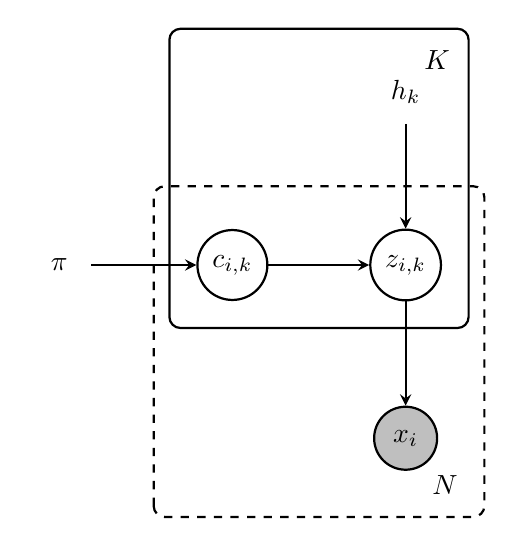
\begin{tikzpicture}[
        obs/.style={circle, draw=black, fill=gray!50, thick, minimum size=8mm},
        lat/.style={circle, draw=black, fill=white, thick, minimum size=8mm},
        param/.style={minimum size=8mm}
    ]
        % Nodes
        \node[param] (pi) at (-2.2, 0) {$\pi$};
        \node[lat] (c) at (0, 0) {$c_{i,k}$};
        \node[lat] (z) at (2.2, 0) {$z_{i,k}$};
        \node[param] (h) at (2.2, 2.2) {$h_k$};
        \node[obs] (x) at (2.2, -2.2) {$x_i$};

        % Edges
        \draw[->, >=stealth, thick] (pi) -- (c);
        \draw[->, >=stealth, thick] (h) -- (z);
        \draw[->, >=stealth, thick] (c) -- (z);
        \draw[->, >=stealth, thick] (z) -- (x);

        % Plate K (Solid)
        \draw[rounded corners, thick] (-0.8, -0.8) rectangle (3.0, 3.0);
        \node at (2.6, 2.6) {$K$};

        % Plate N (Dashed)
        \draw[rounded corners, thick, dashed] (-1.0, -3.2) rectangle (3.2, 1.0);
        \node at (2.7, -2.8) {$N$};

    \end{tikzpicture}
    \caption{Probabilistic Graphical Model of the generative process. Unshaded nodes represent latent variables, shaded nodes represent observed variables, and unboxed text represents deterministic global parameters. The solid rectangle denotes replication over $K$ concepts, while the dashed rectangle denotes replication over $N$ observations in the dataset.}
    \label{fig:pgm}
\end{figure}

\subsection{Inference Model}

Exact inference requires marginalizing over the continuous $z$ and summing over all $2^K$ possible discrete mask configurations for $c$. To maintain tractability, we employ amortized variational inference via an encoder $f_\theta(x)$ that predicts the shared parameters for the latent variables.

\textbf{Embedding Posterior:} \\
We freeze the posterior variance to a constant hyperparameter $\sigma_0^2$. The continuous embeddings are sampled using the reparameterization trick: $z_k = \mu_k(x) + \sigma_0 \cdot \epsilon$, where $\epsilon \sim \mathcal{N}(0, I)$.
\[
q_\theta(z_k \mid x) = \mathcal{N}(z_k; \mu_k(x), \sigma_0^2 I)
\]

\textbf{Dependent Mask Posterior:} \\
To accurately invert the generative flow ($x \to z \to c$), the inference model derives the Bernoulli parameter $\alpha_k(x)$ directly from the predicted spatial location $\mu_k(x)$. We compute this by evaluating the similarity between $\mu_k(x)$ and the global prototype $h_k$, scaled by an inverse temperature $1/\tau$. As proven in \textbf{Appendix A.1}, this formulation is the mathematically optimal parametric form dictated by the Gated Gaussian prior.
\[
\alpha_k(x) = \operatorname{sigmoid}\!\left(\frac{\operatorname{sim}(\mu_k(x), h_k)}{\tau}\right)
\]
In practice, $1/\tau$ is a single learnable scalar (initialised so that $\tau = 0.1$, clamped to $[1, 100]$ at inference), mirroring the CLIP logit-scale parameterisation; the same scale is applied uniformly to all three similarity metrics defined below.
To enable end-to-end optimization through the discrete mask, we draw the actual latent activation $c_k$ using the continuous Gumbel-Sigmoid relaxation during training, parameterized by a Gumbel temperature $\tau_g$:
\[
c_k \sim \text{Gumbel-Sigmoid}(\alpha_k(x), \tau_g)
\]
\[
q_\theta(c_k \mid x) = \operatorname{Bern}(c_k; \alpha_k(x))
\]

\textbf{Decoder Gating at Training/Inference:} \\
Unlike the generative process --- which first draws $c \sim p(c)$ and then $z \sim p(z \mid c)$, so the sampled $z$ already carries the conditioning on $c$ --- the inference posterior $q_\theta(z_k \mid x)$ does not condition on $c_k$: the encoder always produces $\mu_k(x)$ from $x$ alone. A sample $z_k = \mu_k(x) + \sigma_0 \epsilon$ would therefore pass non-zero signal to the decoder regardless of whether the mask says the concept is active. To enforce that inactive concepts contribute exactly zero signal to the reconstruction, we apply a multiplicative gate before invoking the decoder:
\[
\hat{x} = g_\phi(c \odot z), \qquad z = \mu(x) + \sigma_0 \epsilon.
\]
This is a deterministic preprocessing step applied only at training and amortised-inference time --- it does not change the likelihood form, and forward sampling from the generative model needs no such step. Empirically the gate is load-bearing: without it the soft magnitude penalty $(1 - \alpha)\|\mu\|^2$ derived in \S Evidence Lower Bound is too weak to drive inactive $\mu_k$ toward zero, because the reconstruction gradient keeps inflating them. The gate additionally exposes $c$ as a clean handle for concept-level interventions at inference time (see \S Interventions).

\subsection{Evidence Lower Bound}

The full derivation of the Evidence Lower Bound under the structured variational posterior is in Appendix A.2 (which builds on the optimal mask form derived in Appendix A.1). The ELBO decomposes into three analytic components --- a reconstruction term, a per-sample mask KL, and a conditional embedding KL:

\begin{equation*}
\text{ELBO} = \underbrace{\mathbb{E}_{q(z|x)}\!\left[\log p(x \mid z)\right]}_{\text{Reconstruction}} - \underbrace{\sum_{k=1}^K \mathbb{E}_{q(z_k|x)}\!\left[D_{\mathrm{KL}}(q(c_k \mid z_k) \parallel p(c_k))\right]}_{\text{Mask Prior KL}} - \underbrace{\sum_{k=1}^K \mathbb{E}_{q(c_k|z_k)}\!\left[D_{\mathrm{KL}}(q(z_k \mid x) \parallel p(z_k \mid c_k))\right]}_{\text{Conditional Embedding KL}}
\end{equation*}

\textit{*Note on KL direction: the ELBO relies on the reverse KL divergence $D_{\mathrm{KL}}(q \parallel p)$, rather than the forward KL used in maximum likelihood estimation.}

\paragraph{Design Choices}

Translating the analytical ELBO into a training objective requires a few deviations from a strict negated-ELBO loss, each motivated by interpretability or training practicality rather than mathematical necessity:

\begin{itemize}
    \item \textbf{Per-sample $\to$ batch-wise sparsity.} The analytical per-sample Mask Prior KL $D_{\mathrm{KL}}(q(c_k \mid z_k) \parallel p(c_k))$ would pull each sample's $\alpha_k(x_i)$ toward $\pi$ \emph{independently}, which over-constrains the model: different inputs should activate different concepts. We replace it with a population-level constraint that only requires the batch-average $\bar{\alpha}_k = \tfrac{1}{B}\sum_i \alpha_k(x_i)$ to match $\pi$,
    \[
        \beta \sum_{k=1}^K D_{\mathrm{KL}}(\bar{\alpha}_k \parallel \pi),
    \]
    which still penalises "dead" concepts (whose $\bar{\alpha}_k$ collapses across the dataset) but allows individual samples to make confident on/off decisions.

    \item \textbf{Entropy binarisation penalty.} The batch-wise sparsity does not enforce per-sample binarisation: $\alpha_{i,k}$ values clustered around $\pi$ would satisfy it while remaining \emph{soft}. We add
    \[
        \lambda_{\text{ent}}\, \mathcal{H}(\alpha_{i,k}) = -\lambda_{\text{ent}}\bigl[\alpha_{i,k}\log\alpha_{i,k} + (1-\alpha_{i,k})\log(1-\alpha_{i,k})\bigr],
    \]
    which is maximal at $\alpha=1/2$ and zero at the binary extremes; minimising it drives $\alpha$ toward $\{0,1\}$. The motivation is interpretability and alignment with the binary nature of $c$ in the prior --- this is a practical add-on, not a rearrangement of an ELBO term.

    \item \textbf{Mean reductions over $K$ and the embedding dimension $d$.} The factors $1/(BD)$, $1/(BKd)$, $1/(BK)$, $1/K$ in the loss below make each term's magnitude independent of the model dimensions, so the same $\gamma, \beta, \lambda_{\text{ent}}$ values transfer across architectures of different sizes without rescaling.

    \item \textbf{Stop-gradient on $\alpha$.} The $\mathrm{sg}(\cdot)$ operator (\texttt{.detach()}) inside the conditional embedding KL prevents the network from driving $\alpha_{i,k} \to 0$ solely to minimise the $\gamma$ structural penalty. (Appendix~A.2 covers its additional load-bearing role in restoring the closed-form KL under the structured factorisation.)
\end{itemize}

\paragraph{Practical Loss}

Applying the design choices above to the negated ELBO --- and substituting the closed-form conditional embedding KL derived in Appendix~A.2 ($\alpha_{i,k}\|\mu_{i,k} - h_k\|^2 + (1-\alpha_{i,k})\|\mu_{i,k}\|^2$) --- yields:

\begin{equation}
    \begin{aligned}
        \mathcal{L} &= \frac{1}{B D} \sum_{i=1}^B \|x_i - \hat{x}_i\|^2
        + \frac{\gamma}{B K d} \sum_{i=1}^B \sum_{k=1}^K \left( \text{sg}(\alpha_{i,k}) \|\mu_{i,k} - h_k\|^2 + (1 - \text{sg}(\alpha_{i,k})) \|\mu_{i,k}\|^2 \right) \\
        &+ \frac{\lambda_{\text{ent}}}{B K} \sum_{i=1}^B \sum_{k=1}^K \mathcal{H}(\alpha_{i,k})
        + \frac{\beta}{K} \sum_{k=1}^K D_{\mathrm{KL}}(\bar{\alpha}_k \parallel \pi)
    \end{aligned}
\end{equation}

\noindent \textit{where $\hat{x}_i = g_\phi(z_i \odot c_i)$ is the stochastic reconstruction under the inference-time gate of \S Inference Model, and $\mathcal{H}(\alpha) = -[\alpha \log(\alpha) + (1-\alpha) \log(1-\alpha)]$ is the binary entropy function.}

\subsection{Similarity Metrics}

We formulate the mask probability $\alpha_k$ using variants of the generalized $\operatorname{sim}(\cdot)$ function. Since we decode with unnormalized vectors, these metric choices dictate whether the gating mechanism is algebraically coupled to the embedding magnitude.

\begin{table}[h]
\centering
\renewcommand{\arraystretch}{1.5}
\begin{tabular}{>{\bfseries}l c c p{6cm}}
\toprule
Metric & Formulation ($L_k$) & Role of $\tau$ & Properties \\
\midrule
Cosine Similarity & $\frac{1}{\tau} \frac{\mu_k \cdot h_k}{\Vert \mu_k \Vert \Vert h_k \Vert}$ & \textbf{Mandatory} & Bounded. Angle solely controls the discrete gate, while magnitude provides expressivity to the continuous decoder. \\
Inner Product & $\frac{\mu_k \cdot h_k}{\tau}$ & \textbf{Redundant} & Unbounded. Entangles gating directly with continuous expressivity; network can artificially scale $\Vert \mu_k \Vert$. \\
Neg. Euclidean & $\frac{b - \Vert \mu_k - h_k \Vert}{\tau}$ & \textbf{Structural} & Direct geometric fit for the Gaussian prior. Requires learning the radius bias $b$. \\
\bottomrule
\end{tabular}
\end{table}

\subsection{Implementation Details}

\paragraph{Architecture}
A standard backbone (e.g., ResNet, ViT) extracts dense visual features, followed by $K$ distinct linear layers to produce the continuous means $\mu_1, \dots, \mu_K$.

\paragraph{Batch Sparsity}
The global sparsity penalty is evaluated over the batch: $D_{\mathrm{KL}}(\bar{\alpha}_k \parallel \pi)$, where $\bar{\alpha}_k = \frac{1}{B} \sum_{i=1}^B \alpha_k(x_i)$.

\paragraph{Prototype Maintenance}
We do not $L_2$-normalize $h_k$ after optimization steps. Because the active penalty is $\|\mu_{i,k} - h_k\|^2$, allowing the optimizer to freely scale $h_k$ ensures the decoder has access to dynamically sized magnitudes.

\paragraph{Binarization Pressure}
The batch-wise KL divergence lacks a per-sample force to push individual probabilities toward strict bounds. We incorporate a per-sample entropy minimization penalty $\mathcal{H}$ to prevent the model from settling on ambiguous probabilities ($\alpha_{i,k} \approx 0.5$).

\subsection{Interventions}

A central motivation for this formulation is to enable clean concept-level interventions. Standard SAEs require hundreds of concurrently active features to reconstruct a sample, so any meaningful intervention must modify many features at once and risks pushing the latent off-distribution. Our model uses a small number of rich concepts per sample, each pinned to a learned prototype $h_k$, so a single-concept intervention is both semantically meaningful and stays in-distribution. We support two basic operations.

\paragraph{Removal ($c_k \leftarrow 0$)}
Setting $c_k = 0$ forces the decoder input at slot $k$ to exactly zero; the value of $z_k$ becomes irrelevant.

\paragraph{Insertion ($c_k \leftarrow 1$)}
Setting $c_k = 1$ requires also choosing $z_k$. The encoder's $\mu_k(x)$ is unsuitable: for a concept the model judged inactive on this input, the magnitude term $(1 - \alpha_k)\|\mu_k\|^2$ has pushed $\mu_k$ toward $0$, far from the prototype $h_k$. The principled choice, matching what the generative model emits under $c_k = 1$, is to sample from the active prior:
\[
z_k \sim \mathcal{N}(h_k, \sigma_0^2 I).
\]
Sampling produces a distribution of plausible counterfactuals, which is useful when one wants to explore multiple realisations of "concept $k$ active" for the same input. For controlled experiments where reproducibility matters (same input plus same intervention $\Rightarrow$ same output), we collapse the variance and use the prior mean directly, $z_k \leftarrow h_k$.

\textit{Limitations and extensions.} Slots $j \ne k$ retain $\mu_j(x)$ rather than being recomputed under the counterfactual $\mathrm{do}(c_k = 1)$, a lazy approximation shared with standard Concept Bottleneck Model interventions; the strict-causal counterpart requires causal-graph-learning machinery beyond our scope. Continuous modulation, via fractional $c_k \in (0, 1)$ or convex combinations $z_k \leftarrow (1{-}\lambda)\mu_k(x) + \lambda h_k$, is a natural extension for sensitivity studies but not pursued here.

\subsection{Latent Representation Topologies}

The model can be instantiated in two mathematically distinct topologies depending on how the active concept embeddings $c_k z_k$ are passed to the downstream decoder $g_\phi$.

\paragraph{1. Summed Representation ($\sum_{k} c_k z_k \in \mathbb{R}^d$)}
In this topology, the decoder receives a dense, aggregated vector. The model algebraically behaves as a \textbf{Factorial Mixture Model}. 
\begin{itemize}
    \item \textbf{Superposition:} Concepts share a single coordinate system. The decoder processes a linear superposition of features.
    \item \textbf{Capacity \& Interference:} Representational capacity scales combinatorially ($2^K$ states). However, summing introduces the geometric risk of destructive interference. To utilize this topology effectively, the decoder must be capable of algebraically un-mixing overlapping prototypes.
\end{itemize}

\paragraph{2. Stacked Representation ($[c_1 z_1, \dots, c_K z_K] \in \mathbb{R}^{K \times d}$)}
In this topology, the active concepts are stacked into a sequence or structured matrix. 
\begin{itemize}
    \item \textbf{Semantic Isolation:} The concepts are placed into strictly isolated semantic slots. The decoder processes each concept via independent parameter channels.
    \item \textbf{Architectural Orthogonality:} Because the concepts do not share the same algebraic coordinate space, there is zero risk of destructive interference. This topology effectively acts as $K$ parallel, fully disentangled 2-component mixture models.
\end{itemize}

\subsection{Decoder Identifiability}

To ensure that distinct latent slots map to independent visual features and to guarantee generative identifiability, we apply an explicit structural prior to the decoder's weights. 

Assuming a strictly \textbf{linear decoder} (or analyzing the first hidden mixing layer of an MLP), the stacked latent tensor $Z = [c_1 z_1, \dots, c_K z_K]$ is projected via a weight matrix $W$. We partition this matrix into $K$ independent blocks $W = [W_1, W_2, \dots, W_K]$, where each block $W_k$ acts as the explicitly defined visual basis for Concept $k$:
\[
\hat{x} = \sum_{k=1}^K W_k (c_k z_k)
\]
To prevent redundant bases and enforce functional diversity across the dictionary, we introduce a Frobenius orthogonality penalty between these weight blocks, averaged over the $\binom{K}{2}$ pairs so the magnitude of the penalty is invariant to $K$:
\[
\mathcal{L}_{\text{dec\_ortho}} = \frac{\lambda_{\text{ortho}}}{\binom{K}{2}} \sum_{i < j} \frac{\| W_i^T W_j \|_F^2}{\|W_i\|_F^2 \|W_j\|_F^2}
\]
From a Bayesian perspective, this penalty corresponds to Maximum A Posteriori (MAP) estimation under a structural prior $p(\phi)$ that heavily favors orthogonal basis weights. Mathematically forbidding $W_i$ and $W_j$ from mapping to the same downstream features fundamentally prevents capacity cannibalization. Once the network is restricted from using redundant slots to reconstruct high-frequency modes, the optimizer naturally allocates freed slots to span the remaining unexplained variance in the dataset.

\subsection{Related Work}

Our probabilistic formulation conceptually bridges several established paradigms in representation learning, structurally formalizing the relationships between discrete routing and continuous generation.

\paragraph{Concept Embedding Models (CEMs)} 
While standard Variational Autoencoders (VAEs) utilize a dense, highly entangled continuous latent space, our framework establishes a structured bottleneck. It shares lineage with CEMs, which attach high-dimensional continuous embeddings to discrete semantic concepts. However, whereas CEMs traditionally rely on supervised concept labels to regularize these embeddings, our Gated Gaussian framework operates entirely probabilistically, supporting unsupervised or weakly-supervised concept discovery via the evidence lower bound (ELBO).

\paragraph{Vector-Quantized Autoencoders (VQ-VAEs)}
Our framework provides a probabilistic counterpart to discrete quantization models like VQ-VAEs, but with inverted routing mechanisms. A VQ-VAE routes categorical (one-hot) decisions into \textit{spatial} slots using rigid codebook vectors, limiting the representational capacity of a single bottleneck to $K$ discrete states. In contrast, our framework routes independent Bernoulli probabilities into isolated \textit{semantic} slots using gated continuous distributions. This preserves the high-fidelity expressivity and uncertainty handling of continuous VAEs while achieving the interpretable routing of discrete bottlenecks. 

\paragraph{Basis Decomposition and Semantic Embeddings}
Models such as Interpretable Basis Decomposition (IBD) and Knowledge Graph (KG) Embeddings project features into a shared, dense coordinate space where representations are formed via algebraic combinations. In these shared spaces, concepts risk destructive interference (polysemy entanglement) and typically require heavy geometric regularization. Our \textit{Stacked} topology naturally circumvents this entanglement by treating concepts as parallel, structurally orthogonal mixture models, explicitly avoiding the un-mixing problem inherent to linearly summed latent spaces.

\appendix
\section{Mathematical Derivations}

\subsection{Optimal Gating Mechanism (Derivation of $\alpha$)}
To mathematically justify the similarity-based gating, we can derive the optimal form of the mask posterior directly from the generative priors using Bayes' rule. Because $c_k$ is binary, the posterior $p(c_k = 1 \mid z_k)$ is fully characterised by its log-odds, since the sigmoid is the inverse of the logit transform:
\[
p(c_k = 1 \mid z_k) \;=\; \operatorname{sigmoid}\!\left( \log \frac{p(c_k = 1 \mid z_k)}{1 - p(c_k = 1 \mid z_k)} \right) \;=\; \operatorname{sigmoid}\!\left( \log \frac{p(c_k = 1 \mid z_k)}{p(c_k = 0 \mid z_k)} \right).
\]
Computing the posterior probability therefore reduces to computing its log-odds, which by Bayes' rule expand into a tractable function of the priors and likelihoods:

\[
\log \frac{p(c_k = 1 \mid z_k)}{p(c_k = 0 \mid z_k)} = \log \frac{p(z_k \mid c_k = 1) p(c_k = 1)}{p(z_k \mid c_k = 0) p(c_k = 0)}
\]

Splitting the right-hand side into a likelihood ratio and a prior ratio gives:
\[
\text{Log-Odds} = \underbrace{\log \frac{p(z_k \mid c_k = 1)}{p(z_k \mid c_k = 0)}}_{\text{likelihood ratio}} + \underbrace{\log \frac{p(c_k = 1)}{p(c_k = 0)}}_{= \log \frac{\pi}{1-\pi} \,=\, \operatorname{logit}(\pi)}
\]

The prior ratio is just the logit of the Bernoulli activation probability $\pi$. For the likelihood ratio we substitute the Gated Gaussian densities $p(z_k \mid c_k = 1) = \mathcal{N}(z_k; h_k, I)$ and $p(z_k \mid c_k = 0) = \mathcal{N}(z_k; 0, I)$. The two distributions share the same isotropic covariance, so the $(2\pi)^{-d/2}$ normalising constants cancel inside the log-ratio:
\[
\log \frac{p(z_k \mid c_k = 1)}{p(z_k \mid c_k = 0)}
\;=\;
\log \frac{\exp\!\left(-\tfrac{1}{2}\|z_k - h_k\|^2\right)}{\exp\!\left(-\tfrac{1}{2}\|z_k\|^2\right)}
\;=\;
-\tfrac{1}{2}\|z_k - h_k\|^2 + \tfrac{1}{2}\|z_k\|^2.
\]

Adding the prior log-odds back in yields:

\[
\text{Log-Odds} = -\frac{1}{2}\|z_k - h_k\|^2 + \frac{1}{2}\|z_k\|^2 + \operatorname{logit}(\pi)
\]

By algebraically expanding the squared distance ($\|z_k - h_k\|^2 = \|z_k\|^2 - 2 z_k^T h_k + \|h_k\|^2$), the $\frac{1}{2}\|z_k\|^2$ terms perfectly cancel out:

\[
\text{Log-Odds} = z_k^T h_k - \frac{1}{2}\|h_k\|^2 + \operatorname{logit}(\pi)
\]

Converting the log-odds back to a probability via the sigmoid function, and substituting the encoder's predicted mean $\mu_k$ for $z_k$, we recover an inner-product formulation that is exact under the Gated Gaussian prior:

\[
\alpha_k = \operatorname{sigmoid}\!\left( \mu_k^T h_k - \tfrac{1}{2}\|h_k\|^2 + \operatorname{logit}(\pi) \right)
\]

In the implementation we drop the additive constants $-\tfrac{1}{2}\|h_k\|^2 + \operatorname{logit}(\pi)$ and parameterise the logit as $(1/\tau)\,\mu_k^T h_k$, where the per-prototype bias is left to be absorbed implicitly into the learnable inverse temperature and the optimisation of $h_k$ itself. Concretely, the decision threshold sits at $\mu_k = \tfrac{1}{2}h_k$, which is well-calibrated as long as $\|\mu_k\| \approx \|h_k\|$; otherwise the model can ``cheat'' by inflating $\|\mu_k\|$ to push the inner product up. The cosine-similarity variant of \S\,Similarity Metrics removes this magnitude coupling by construction.

%Or if we consider $||h_k||^2 \approx ||\mu_k|| ||h_k|| $, we can recover a cosine similarity:
%\[
%\alpha_k \approx \operatorname{sigmoid}\left( \frac{1}%{2}\frac{\mu_k^T h_k}{||\mu_k|| ||h_k||}\right),
%\]
%which avoids magnitude issues related to $\mu_k$. 


This proves that tying a concept's probability of being active ($\alpha_k$) to its spatial proximity to its prototype ($h_k$) is not an arbitrary heuristic, but the optimal parametric form dictated by the Gated Gaussian prior.

\subsection{Explicit ELBO Derivation}

To maximize the log marginal likelihood of the data $\log p(x)$, we introduce the approximate posterior $q(c, z \mid x)$ and apply Jensen's Inequality to derive the Evidence Lower Bound (ELBO).

\textbf{Step 1: The Lower Bound}\\
To compute the log marginal likelihood of the data $\log p(x)$, we must marginalize over all possible latent states. Because this integral over the continuous $z$ and sum over the discrete $c$ is computationally intractable, we introduce our approximate posterior $q(c, z \mid x)$ and multiply the integrand by $1 = \frac{q(c, z \mid x)}{q(c, z \mid x)}$:

\[
\log p(x) = \log \sum_c \int p(x, c, z) \frac{q(c, z \mid x)}{q(c, z \mid x)} \, dz
\]

This allows us to mathematically rewrite the expression as an expectation over our approximate posterior:

\[
\log p(x) = \log \left( \mathbb{E}_{q(c, z \mid x)}\left[ \frac{p(x, c, z)}{q(c, z \mid x)} \right] \right)
\]

Because the logarithm is a concave function, we can apply \textbf{Jensen's Inequality} ($\log \mathbb{E}[Y] \ge \mathbb{E}[\log Y]$) to move the logarithm inside the expectation. This bounds the log-likelihood from below, giving us the Evidence Lower Bound (ELBO) that we can maximize:

\[
\log p(x) \ge \mathbb{E}_{q(c, z \mid x)}\left[\log \frac{p(x, c, z)}{q(c, z \mid x)}\right] \equiv \text{ELBO}
\]

\textbf{Step 2: Factorizing the Distributions}\\
Based on our hierarchical generative model, the joint distribution factorizes over the independent concepts as:

\[
p(x, c, z) = p(x \mid z) \prod_{k=1}^K p(c_k) p(z_k \mid c_k)
\]

Mirroring the optimal $q(c \mid z)$ derived in Appendix A.1, we adopt a \emph{structured} variational posterior in which $c$ is conditioned on $z$ rather than directly on $x$:

\[
q(c, z \mid x) = \prod_{k=1}^K q(c_k \mid z_k) \, q(z_k \mid x)
\]

In practice, the inference network evaluates $q(c_k \mid z_k)$ at the posterior mean $z_k = \mu_k(x)$, so that $\alpha_k = q(c_k = 1 \mid z_k = \mu_k(x))$ becomes a deterministic function of $\mu_k(x)$. The stop-gradient $\mathrm{sg}(\alpha)$ in the practical loss then severs the dependence of $\alpha$ on the sampled $z$ inside the inner expectation, which restores the closed-form per-sample KL we derive below.

\textbf{Step 3: Expanding the Expectation}\\
First, we substitute the factorized distributions directly into the ELBO fraction:

\[
\text{ELBO} = \mathbb{E}_{q(c, z \mid x)} \left[ \log \frac{p(x \mid z) \prod_{k=1}^K p(c_k) p(z_k \mid c_k)}{\prod_{k=1}^K q(c_k \mid z_k) q(z_k \mid x)} \right]
\]

Because the products in the numerator and denominator share the same index $k$, we can group the terms inside a single product block:

\[
\text{ELBO} = \mathbb{E}_{q(c, z \mid x)} \left[ \log \left( p(x \mid z) \prod_{k=1}^K \frac{p(c_k)}{q(c_k \mid z_k)} \frac{p(z_k \mid c_k)}{q(z_k \mid x)} \right) \right]
\]

Next, using the properties of logarithms ($\log(A \cdot B) = \log A + \log B$ and $\log \prod A_k = \sum \log A_k$), the logarithm converts the multiplication into addition and the product into a sum, cleanly separating the likelihood from the concept distributions:

\[
\text{ELBO} = \mathbb{E}_{q(c, z \mid x)} \left[ \log p(x \mid z) + \sum_{k=1}^K \log \frac{p(c_k)}{q(c_k \mid z_k)} + \sum_{k=1}^K \log \frac{p(z_k \mid c_k)}{q(z_k \mid x)} \right]
\]

\textbf{Step 4: Grouping into KL Divergences}\\
By linearity of expectation, and using the structured factorisation $\mathbb{E}_{q(c, z \mid x)} = \mathbb{E}_{q(z \mid x)} \mathbb{E}_{q(c \mid z)}$, we separate the ELBO into three components:

\begin{enumerate}
    \item \textbf{Reconstruction Term:}
    \[
    \mathbb{E}_{q(z \mid x)}[\log p(x \mid z)]
    \]

    \item \textbf{Mask Prior KL:} Because $q(c_k \mid z_k)$ depends on the sampled $z_k$, the per-sample mask KL is itself an expectation over $q(z_k \mid x)$:
    \[
    \sum_{k=1}^K \mathbb{E}_{q(z_k \mid x)} \mathbb{E}_{q(c_k \mid z_k)} \!\left[ \log \frac{p(c_k)}{q(c_k \mid z_k)} \right] = - \sum_{k=1}^K \mathbb{E}_{q(z_k \mid x)} \!\left[ D_{\mathrm{KL}}(q(c_k \mid z_k) \parallel p(c_k)) \right]
    \]

    \item \textbf{Conditional Embedding term:} The remaining term does \emph{not} factor as a single KL because $q(z_k \mid x)$ is not conditioned on $c_k$:
    \[
    \sum_{k=1}^K \mathbb{E}_{q(z_k \mid x)} \mathbb{E}_{q(c_k \mid z_k)} \!\left[ \log \frac{p(z_k \mid c_k)}{q(z_k \mid x)} \right].
    \]
    The closed form is recovered by treating $q(c_k \mid z_k)$ as a fixed Bernoulli with parameter $\alpha_k = q(c_k = 1 \mid z_k = \mu_k(x))$ inside the inner expectation --- i.e., the stop-gradient $\mathrm{sg}(\alpha)$ of \S Evidence Lower Bound. Under this approximation the inner expectation factors and we obtain
    \[
    -\sum_{k=1}^K \!\left[ \alpha_k\, D_{\mathrm{KL}}(q(z_k \mid x) \parallel p(z_k \mid c_k{=}1)) + (1-\alpha_k)\, D_{\mathrm{KL}}(q(z_k \mid x) \parallel p(z_k \mid c_k{=}0)) \right]
    \]
    which evaluates analytically (variance constants cancel) to the $\alpha_k \|\mu_k - h_k\|^2 + (1-\alpha_k)\|\mu_k\|^2$ form used in the Practical Loss of \S Evidence Lower Bound.
\end{enumerate}

\textbf{Step 5: The Final Analytical ELBO}\\
Combining the terms (under the $\mathrm{sg}(\alpha)$ approximation discussed above), the Evidence Lower Bound to maximise is:

\[
\text{ELBO} = \underbrace{\mathbb{E}_{q}[\log p(x \mid z)]}_{\text{Reconstruction}} - \underbrace{\sum_{k=1}^K \mathbb{E}_{q(z_k \mid x)}\!\left[ D_{\mathrm{KL}}(q(c_k \mid z_k) \parallel p(c_k)) \right]}_{\text{Mask Prior KL}} - \underbrace{\sum_{k=1}^K \mathbb{E}_{q(c_k \mid z_k)} \!\left[ D_{\mathrm{KL}}(q(z_k \mid x) \parallel p(z_k \mid c_k)) \right]}_{\text{Conditional Embedding KL}}
\]

\vspace{0.5cm}
\noindent \textbf{Connection to Our Practical Loss Objective ($\mathcal{L}$):}\\
The training objective in \S Evidence Lower Bound is obtained by negating this analytical ELBO and applying the design choices listed there (batch-wise sparsity in place of the per-sample mask KL, entropy binarisation penalty, mean reductions over $K$ and $d$, and stop-gradient on $\alpha$).

\end{document}